% !TeX root = ../report.tex

\section{Trident Ray Theory}

Currently, there are many existing ray tracing algorithms for High-Intensity Focused Ultrasound simulation. All of them aim at computing the powerloss density (heat production) or intensity from beams of rays casted from transducer. 

The first method is to sum over all rays (set $\Phi$) that pass through a grid cube. Their energy loss in the cube is:

\begin{equation} \label{eq:first_rc}
    H = \sum_{a \in \Phi} (P(r_{a,in}) - P(r_{a,out})) = \sum_{a \in \Phi} P(r_{a,in})(1-e^{-2\alpha ||r_{a,in} - r_{a,out}||})
\end{equation}

Here $H$ is the total powerloss by all rays in the sampling grid. To obtain the powerloss density $Q$ (in $watt/m^3$), we need to divide $H$ by volume. For each ray in $\Phi$, we need to calculate the position where it enters and leaves a gridbox. Take the situation in Figure \ref{fig:one_gridbox} for example, the the value of the intensity loss for the all the rays that follow the same path can be calculated from: 

$$I_{loss,\Phi}(\vec{r_c})=\sum_{a \in \Phi} \frac{||\vec{r}_{a,in}-\vec{r}_{a,out}||}{V} P(\vec{r}_{a,in})$$
\label{eq:calc_I_Loss}

From intensity loss $I_{loss}$, pressure generated by the rays in the same path can be calculated from:

$$p_b(\vec{r}_c)=\sqrt{2\cdot Z\cdot I_{loss,b}(\vec{r}_c)e^{i\bar{\phi}_b}}$$

Note that here same path only means that the rays pass through the media in the same order and have same properties such as wave type. Ray with the same path are treated as a bundle. We do the calculation above for all the possible paths and sum up the results:

$$p_{tot}(\vec{r}_c)=\sum_{b \in U}p_b(\vec{r}_c)$$

From Daniela et al \cite{Modena_2018}, the fluid heat production is given by:
$$Q(\vec{r})=\frac{\alpha}{Z}|p_{tot}|^2$$
\label{eq:fluid_hp}

\begin{figure}
    \centering
    \begin{subfigure}[b]{0.45\textwidth}
        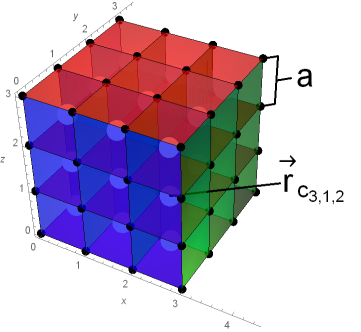
\includegraphics[width=\textwidth]{gridbox}
        \caption{$r_c$ is the center of the box}
        \label{fig:gridbox}
    \end{subfigure}
    %
    \begin{subfigure}[b]{0.5\textwidth}
        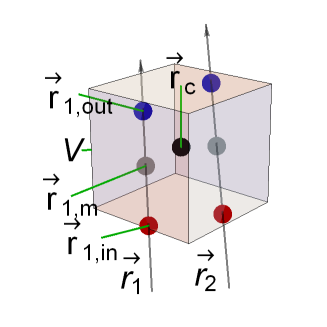
\includegraphics[width=\textwidth]{one_gridbox}
        \caption{$r_1$ enters the box at $r_{1,in}$ and exit at $r_{1,out}$, similar for $r_2$}
        \label{fig:one_gridbox}
    \end{subfigure}
    \caption{(a) An example of Axis-Aligned Bounding Box (AABB) and (b) single box with intersection}
\end{figure}

Combining, the above equations, we can arrive at the equation for heat production calculated from ultrasonic rays.
$$Q(\vec{r}_c)=\frac{2\alpha}{V}\left|\sum_{b \in U}\sqrt{(\sum_{a \in U_b}P(\vec{r}_{a,in})\left\|\vec{r}_{a,in}-\vec{r}_{a,out}\right\|)} e^{i\bar{\phi}_b}\right|^2$$

To obtain the powerloss density, first, within every path (bundle), the impact of all the rays are accumulated. For every path, their contribution is also calculated in the outer summation. This causes the computation to be very expensive when there are a large number of rays to approximate the real intensity.

A new idea is proposed by Prof. Huub ten Eikelder that instead of casting many rays from the transducer to approximate the intensity, one can use a "trident" ray, a combination of three rays to keep track of the spreading of the beam. One of the three rays carrys the power information, the other two only serve as auxiliary rays. These three rays have almost identical paths and the geometrical spreading can be used as the divergence of the ray pattern. At a certain point, a plane perpendicular to the power carrying ray is created to intersect the three rays. The area of the triangle formed by the three intersection points is $S_1$ and can be used as how much the beam has spreaded. The power of the ray is given by attenuation equation $P_1=P_0\cdot e^{-2\cdot \alpha \cdot r}$. Hence, the intensity and powerloss density can be derived from:
$$I=\frac{P_1}{S_1}, Q=2\alpha I$$
This method can achieve similar pricision with less rays, compared with the first method.

\begin{figure}
    \centering
    \includegraphics[width=0.6\textwidth]{untitled.eps}
    \caption{An example of trident rays, the angle between rays are larger for demonstration only}
    \label{fig:Trident_ray}
\end{figure}

\section{Components of HIFU System}
markoil \cite{markoil}
\section{Implementation of the Model}
matplotlib\cite{matplotlib}
scipy suite\cite{scipy}

\section{Visualization}